\documentclass{article}

\usepackage{fancyhdr}
\usepackage{extramarks}
\usepackage{amsmath}
\usepackage{amsthm}
\usepackage{amsfonts}
\usepackage{amssymb}
\usepackage{tikz}
\usepackage[plain]{algorithm}
\usepackage{algpseudocode}

\usetikzlibrary{automata,positioning}

%
% Basic Document Settings
%

\topmargin=-0.45in
\evensidemargin=0in
\oddsidemargin=0in
\textwidth=6.5in
\textheight=9.0in
\headsep=0.25in

\linespread{1.1}

\pagestyle{fancy}
\lhead{\hmwkAuthorName}
\chead{\hmwkClass\ (\hmwkClassInstructor): \hmwkTitle}
\rhead{\firstxmark}
\lfoot{\lastxmark}
\cfoot{\thepage}

\renewcommand\headrulewidth{0.4pt}
\renewcommand\footrulewidth{0.4pt}

\setlength\parindent{0pt}

\newcommand\numberthis{\addtocounter{equation}{1}\tag{\theequation}}

%
% Create Problem Sections
%

\newcommand{\enterProblemHeader}[1]{
    \nobreak\extramarks{}{Problem \arabic{#1} continued on next page\ldots}\nobreak{}
    \nobreak\extramarks{Problem \arabic{#1} (continued)}{Problem \arabic{#1} continued on next page\ldots}\nobreak{}
}

\newcommand{\exitProblemHeader}[1]{
    \nobreak\extramarks{Problem \arabic{#1} (continued)}{Problem \arabic{#1} continued on next page\ldots}\nobreak{}
    \stepcounter{#1}
    \nobreak\extramarks{Problem \arabic{#1}}{}\nobreak{}
}

\setcounter{secnumdepth}{0}
\newcounter{partCounter}
\newcounter{homeworkProblemCounter}
\setcounter{homeworkProblemCounter}{1}
\nobreak\extramarks{Problem \arabic{homeworkProblemCounter}}{}\nobreak{}

%
% Homework Problem Environment
%
% This environment takes an optional argument. When given, it will adjust the
% problem counter. This is useful for when the problems given for your
% assignment aren't sequential. See the last 3 problems of this template for an
% example.
%
\newenvironment{homeworkProblem}[1][-1]{
    \ifnum#1>0
        \setcounter{homeworkProblemCounter}{#1}
    \fi
    \section{Problem \arabic{homeworkProblemCounter}}
    \setcounter{partCounter}{1}
    \enterProblemHeader{homeworkProblemCounter}
}{
    \exitProblemHeader{homeworkProblemCounter}
}

%
% Homework Details
%   - Title
%   - Due date
%   - Class
%   - Section/Time
%   - Instructor
%   - Author
%

\newcommand{\hmwkTitle}{Homework\ \#2}
\newcommand{\hmwkDueDate}{October 13, 2016}
\newcommand{\hmwkClass}{CS300}
\newcommand{\hmwkClassInstructor}{Prof. Sunghee Choi}
\newcommand{\hmwkAuthorName}{Ohjun Kwon}

%
% Title Page
%

\title{
    \vspace{2in}
    \textmd{\textbf{\hmwkClass:\ \hmwkTitle}}\\
    \normalsize\vspace{0.1in}\small{Due\ on\ \hmwkDueDate\ at 10:30am}\\
    \vspace{0.1in}\large{\textit{\hmwkClassInstructor}}
    \vspace{3in}
}

\author{\textbf{20160051 \hmwkAuthorName}}
\date{}

\renewcommand{\part}[1]{\textbf{\large Part \Alph{partCounter}}\stepcounter{partCounter}\\}

%
% Various Helper Commands
%

% Useful for algorithms
\newcommand{\alg}[1]{\textsc{\bfseries \footnotesize #1}}

% For derivatives
\newcommand{\deriv}[1]{\frac{\mathrm{d}}{\mathrm{d}x} (#1)}

% For partial derivatives
\newcommand{\pderiv}[2]{\frac{\partial}{\partial #1} (#2)}

% Integral dx
\newcommand{\dx}{\mathrm{d}x}

% Alias for the Solution section header
\newcommand{\solution}{\textbf{\large Solution}}

% Probability commands: Expectation, Variance, Covariance, Bias
\newcommand{\E}{\mathrm{E}}
\newcommand{\Var}{\mathrm{Var}}
\newcommand{\Cov}{\mathrm{Cov}}
\newcommand{\Bias}{\mathrm{Bias}}

\begin{document}

\maketitle

\pagebreak
\begin{homeworkProblem}
\textbf{(a)}
Quicksort is done by partitioning the given array, 
so it's performance can be differ by how the array partitions.
If the given array's length is $n$ and the array is partitioned into two subarrays
whose length are $i$ and $n-i$, we can make a recurrence like below.
$$
T(n)=T(i)+T(n-i-1)+\Theta(n)
$$
We want to prove the best-case running time is $\Omega(n\lg n)$
so we need to calculate the minimum of the recurrence.
$$
T(n)=\min_{0\leq i\leq n-1}(T(i)+T(n-i-1))+\Theta(n)
$$
As we want to prove that running time is $\Omega(n\lg n)$, 
we assume that $T(n)\geq cn\lg n$.
\begin{align*}
T(n)&=\min_{0\leq i\leq n-1}(T(i)+T(n-i-1))+\Theta(n)\\
&\geq \min_{0\leq i\leq n-1}(ci\lg i+c(n-i-1)\lg (n-i-1))+\Theta(n)\\
&=c\cdot \min_{0\leq i\leq n-1}(i\lg i+(n-i-1)\lg (n-i-1))+\Theta(n)
\end{align*}
We have to find $\min_{0\leq i\leq n-1}(i\lg i+(n-i-1)\lg (n-i-1))$ to evaluate the recurrence.
Let $f(x)=x\lg x+(n-x-1)\lg (n-x-1)$.
\begin{align*}
f'(x)&=\frac 1{\ln 2} \left(\ln x + 1 - \ln (n-x-1) - 1\right)\\
&=\frac{\ln x -\ln (n-x-1)}{\ln 2}
\end{align*}
We have to find the minimum of $f(x)$, so we have to find where $f'(x)$ is $0$.
\begin{gather*}
\frac{\ln x -\ln (n-x-1)}{\ln 2}=0\\
\ln x -\ln (n-x-1)=0\\
\ln\frac x{n-x-1}=0\\
\frac x{n-x-1}=1\\
x=n-x-1\\
2x=n-1\\
x=\frac{n-1}2
\end{gather*}
We have found that $x=\frac{n-1}2$ is a critical point, but we don't know whether
the point is a minimum. Therefore, we should check $f''\left(\frac{n-1}2\right)$ in order to confirm that
the point is a minimum.
\begin{align*}
f''(x)&=\frac {df'}{dx} = \frac d{dx}\left(\frac{\ln x -\ln (n-x-1)}{\ln2}\right)\\
&= \frac 1{\ln 2}\left( \frac 1 x + \frac 1 {n-x-1}\right)
\end{align*}
\begin{align*}
f''\left(\frac{n-1}2\right)&=\frac 1{\ln 2}\left(\frac 1{\frac{n-1}2}+\frac 1{n-\frac{n-1}2-1}\right)\\
&=\frac 1{\ln 2}\left(\frac 2{n-1}+\frac 2{2n-n+1-2}\right)\\
&=\frac 1{\ln 2}\left(\frac 2{n-1}+\frac 2{n-1}\right)\\
&=\frac 1{\ln 2}\left(\frac 4{n-1}\right)
\end{align*}
For $n\geq 2$, $f''(\frac{n-1}2)$ is positive. Therefore, the point is a minimum of $f(x)$.
Now, we can plug in $i=\frac{n-1}2$ for establishing the minimum.
\begin{align*}
T(n)&\geq c\cdot \min_{0\leq i\leq n-1}(i\lg i+(n-i-1)\lg (n-i-1))+\Theta(n)\\
&\geq c\left(\frac{n-1}2\lg \frac{n-1}2+\left(n-\frac{n-1}2-1\right)\lg \left(n-\frac{n-1}2-1\right)\right)+\Theta(n)
\label{eq:1}
\numberthis
\\
&= c\left(\frac{n-1}2\lg \frac{n-1}2+\frac{2n-n+1-2}2\lg \frac{2n-n+1-2}2\right)+\Theta(n)\\
&= c\left(\frac{n-1}2\lg \frac{n-1}2+\frac{n-1}2\lg \frac{n-1}2\right)+\Theta(n)\\
&= c(n-1)\lg \frac{n-1}2+\Theta(n)\\
&= c(n-1)\lg (n-1)-c(n-1)+\Theta(n)\\
&= cn\lg (n-1)-c\lg (n-1)-c(n-1)+\Theta(n)\\
&\geq cn\lg \frac n2-c\lg (n-1)-c(n-1)+\Theta(n)\numberthis \label{eq:2}\\
&= cn\lg n-cn-c\lg (n-1)-c(n-1)+\Theta(n)\\
&\geq cn\lg n \numberthis \label{eq:3}
\end{align*}
(\ref{eq:1}): for $n\geq 2$\\
(\ref{eq:2}): for $n\geq 2$
\begin{gather*}
n\geq 2\\
2n-2\geq n\\
n-1\geq \frac n2\\
\lg (n-1)\geq \lg \frac n2
\end{gather*}
(\ref{eq:3}): we can find and set $c$ that satisfies $\Theta(n)-cn-c\lg (n-1)-c(n-1)\geq 0$.

$\therefore T(n)\in \Omega (n\lg n)$ \qedsymbol
\\

\textbf{(b)}
We have shown in class that 
$$
E[T(n)]=\frac 2n \sum_{k=2}^{n-1}E[T(k)]+\Theta(n)
$$
where $T(n)$ is the random variable for the running time of randomized quicksort on an input of size $n$.
We have to show that $E[T(n)]$ is $\Omega(n\lg n)$. Let's assume $E[T(n)]\geq cn\lg n$.
\begin{align*}
E[T(n)]&=\frac 2n \sum_{k=2}^{n-1}E[T(k)]+\Theta(n)\\
&\geq \frac 2n \sum_{k=2}^{n-1}ck\lg k+\Theta(n)\numberthis \label{eq:4} \\
&\geq \frac 2n \int_{1}^{n-1}ck\lg k\  \mbox d k+\Theta(n)\numberthis\label{eq:5}\\
&= \frac 2n \int_{1}^{n-1}\frac c{\ln 2}k\ln k\  \mbox d k+\Theta(n)\\
&= \frac 2n \frac c{\ln 2}\int_{1}^{n-1}k\ln k\  \mbox d k+\Theta(n)\\
&= \frac 2n \frac c{\ln 2}\left[\frac 14 x^2(2\ln x -1)\right]_1^{n-1}+\Theta(n)\\
&= \frac c{2n\ln 2}\left[2x^2\ln x -x^2\right]_1^{n-1}+\Theta(n)\\
&= \frac c{2n\ln 2}\left[2(n-1)^2\ln (n-1) -(n-1)^2 - 1\right]+\Theta(n)\\
&= \frac c{2n\ln 2}\left[2n^2\ln (n-1)-\left((4n-2)\ln (n-1)+(n-1)^2+1\right)\right]+\Theta(n)\\
&= cn\lg (n-1)-\frac c{2n\ln 2}\left((4n-2)\ln (n-1)+(n-1)^2+1\right)+\Theta(n)\\
&\geq cn\lg (n/2)-\frac c{2n\ln 2}\left((4n-2)\ln (n-1)+(n-1)^2+1\right)+\Theta(n)\numberthis \label{eq:6}\\
&= cn\lg n-cn-\frac c{2n\ln 2}\left((4n-2)\ln (n-1)+(n-1)^2+1\right)+\Theta(n)\\
&\geq cn\lg n\numberthis \label{eq:7}
\end{align*}
(\ref{eq:4}): assumption\\
(\ref{eq:5}): in Figure~\ref{fig:1}, each of the area is representing its value that is written besides. We can see that $\sum_{k=2}^{n-1}k\lg k$ is grater than $\int_1^{n-1}x\lg x\mbox{ d}x$.
\begin{figure}[!ht]
	\centering
	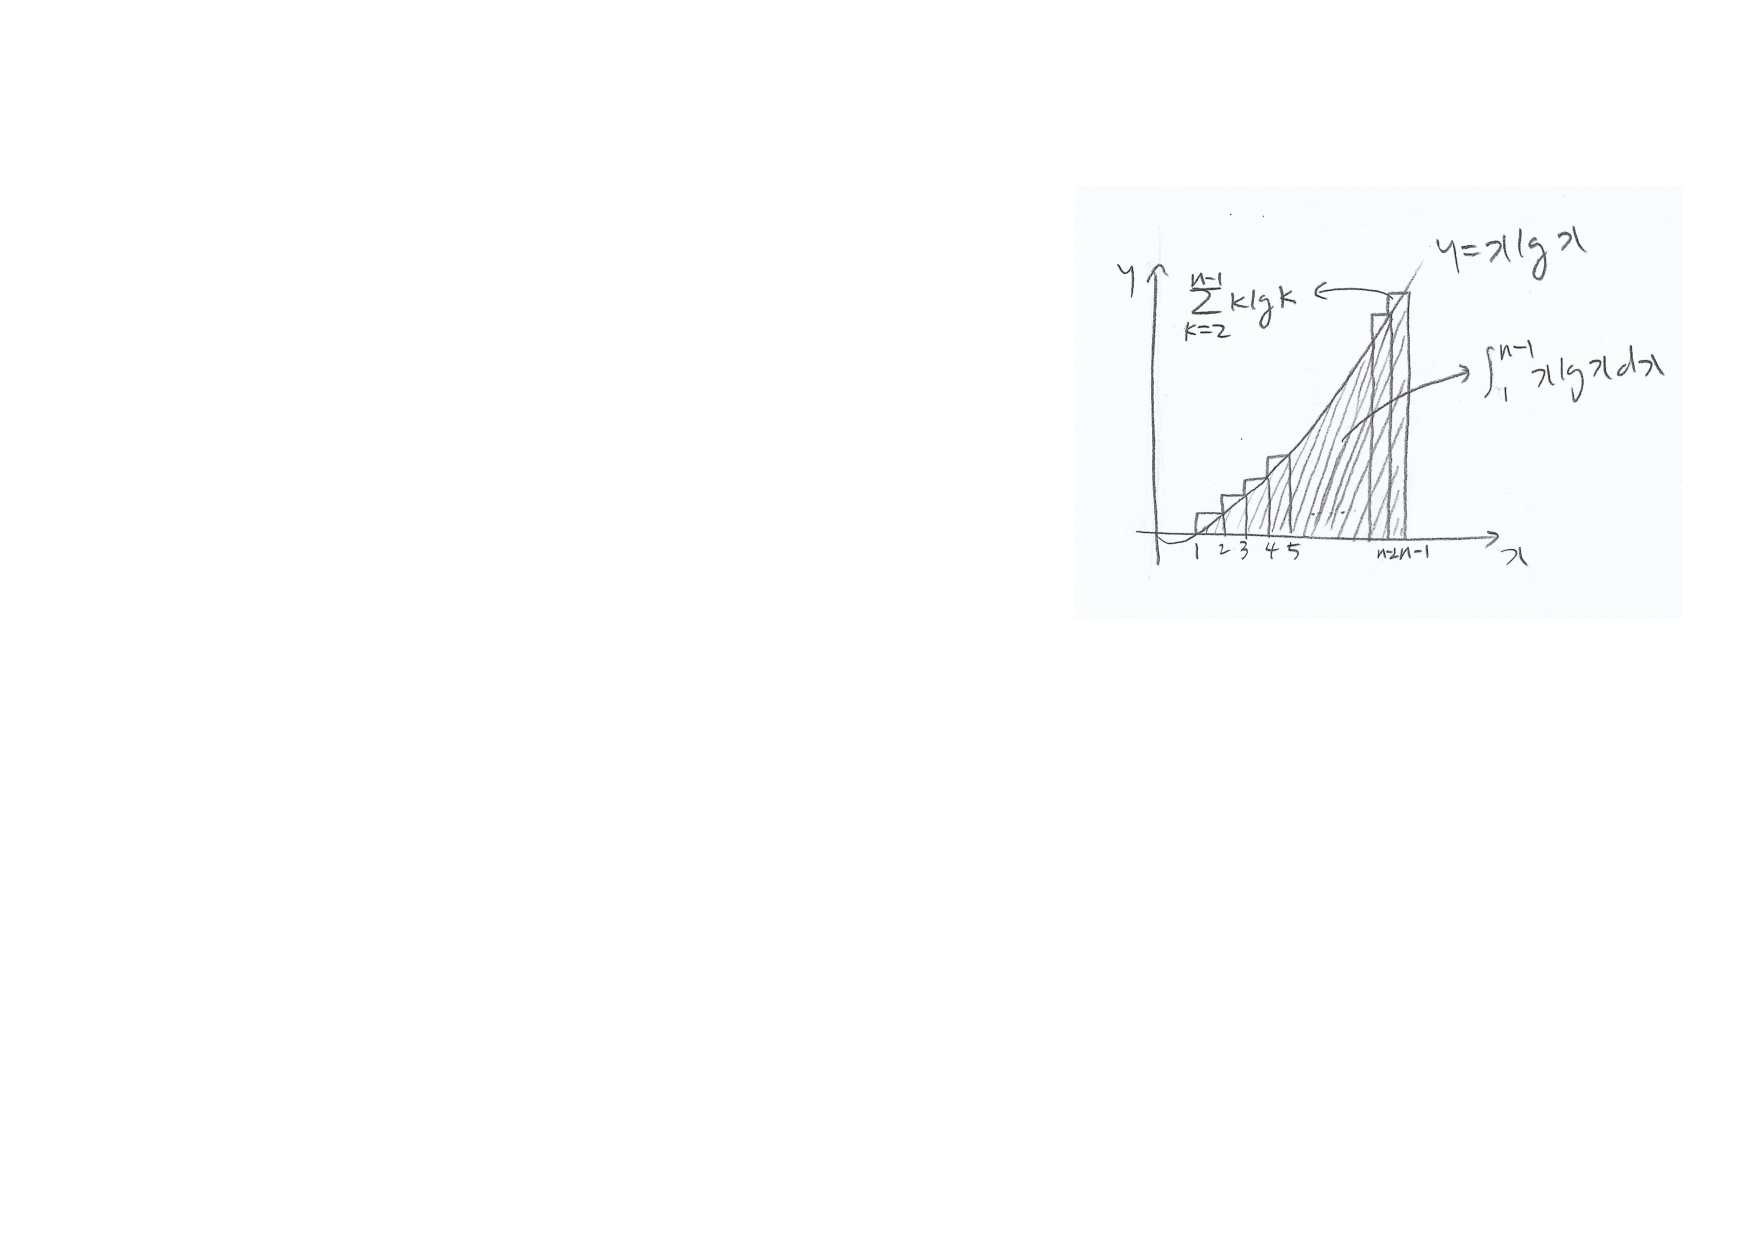
\includegraphics[width=0.5\textwidth]{graph}
	\caption{graph}
	\label{fig:1}
\end{figure}
\\
(\ref{eq:6}): we can prove this in the same way in Equation~\ref{eq:2} for $n\geq 2$\\
(\ref{eq:7}): we can find and set $c$ that satisfies $\Theta(n)-cn-\frac c{2n\ln 2}\left((4n-2)\ln (n-1)+(n-1)^2+1\right)\geq 0$.\\
$\therefore E[T(n)]\in\Omega (n\lg n)$ \qedsymbol
\end{homeworkProblem}

\begin{homeworkProblem}
We have three solving ways in the question. We can make recurrences for each of them.\\
A: $T(n)=3T(n/2)+\Theta(n^2\sqrt n)$\\
B: $T(n)=4T(n/2)+\Theta(n^2)$\\
C: $T(n)=5T(n/2)+\Theta(n\lg n)$\\

\part

$T(n)=3T(n/2)+\Theta(n^2\sqrt n)$\\
$a=3$, $b=2$ $\Rightarrow$ $n^{\log_ba}=n^{\lg 3}$; $f(n)=\Theta(n^2\sqrt n)$\\
Case 3 on the master method: $f(n)\in\Theta(n^{2.5})\subset \Omega(n^2)=\Omega(n^{\lg 3+\epsilon})$, for some $\epsilon > 0$ ($\because 1<\lg 3<2$)\\
and $3(n/2)^{2.5}\leq cn^{2.5}$ $\Rightarrow$ $3/2^{2.5}\leq c < 1$, for some $c<1$\\
$\therefore T(n)=\Theta(n^{2.5})$
\\

\part

$T(n)=4T(n/2)+\Theta(n^2)$\\
$a=4$, $b=2$ $\Rightarrow$ $n^{\log_ba}=n^2$; $f(n)=\Theta(n^2)$\\
Case 2 on the master method: $f(n)=\Theta(n^2\lg^0n)$, $k=0$\\
$\therefore T(n)=\Theta(n^2\lg n)$
\\

\part

$T(n)=5T(n/2)+\Theta(n\lg n)$\\
$a=5$, $b=2$ $\Rightarrow$ $n^{\log_ba}=n^{\lg 5}$; $f(n)=\Theta(n\lg n)$\\
Case 1 on the master method: $f(n)\in \Theta(n\lg n)\subset O(n^2)=O(n^{\lg 5 -\epsilon})$, for some $\epsilon>0$ ($\because 2<\lg 5<3$)\\
$\therefore T(n)=\Theta(n^{lg 5})\approx \Theta(n^{2.32})$
\\

$\therefore T_B(n)<T_C(n)<T_A(n)$, for sufficiently large n.\\

I prefer method B.
\end{homeworkProblem}

\begin{homeworkProblem}
We are taking advantage of insertion sort's fast running time when the input data size is small, so the quicksort will be halted when the partitioned subarray's size is less than k. The quicksort will be stop at $O(\lg(n/k))$, so the expected running time is $O(n\lg (n/k))$. The unsorted part will be sorted by the insertion sort. There are $O(n/k)$ unsorted subarrays and its size is $O(k)$, and the insertion sort's expected running time is $O(n^2)$. Therefore, the insertion sort part's expected running time is $O((n/k)k^2)=O(nk)$. In conclusion, the given sorting algorithm sorts the data in $O(nk+n\lg (n/k))$. Theoretically, We can calculate the factor $k$ approximately by solving inequality Equation~\ref{eq:8}.
\begin{equation}
c_1\left(nk+n\lg \frac nk\right)\leq c_2(n\lg n)
\label{eq:8}
\end{equation}
where $c_1$ and $c_2$ are constant factors. In practice, we should pick the factor $k$ by performing the actual experiments.
\end{homeworkProblem}
\end{document}
